\documentclass[11pt,a4paper]{article}
\usepackage[utf8]{inputenc}
\usepackage[round]{natbib}
%\usepackage[style=authoryear,sorting=ynt]{biblatex}
\bibliographystyle{plainnat}
\usepackage[hyperref]{acl2018}
\usepackage{times}
\usepackage{latexsym}
\usepackage{url}
\usepackage{array}
\usepackage{graphicx}
\usepackage[font=small,labelfont=bf]{caption}
\graphicspath{ {./img/} } 
\pagestyle{plain}

\title{{\LARGE Advances and Problems in Reinforcement Learning for Natural Language Processing}\\[1.5mm]
{\large Final paper: Literature Review Article}\\[1.5mm]} 
\author{Author: Lisa Becker (775242) } 

\begin{document}
\maketitle
\section{Abstract}


\section{Introduction}
In 2016, DeepMind put Reinforcement Learning (RL) in the spotlights by developing AlphaGo \citep{alphago}. Since then, RL has made many advantages in various subdomains, one of them being Natural Language Processing (NLP). As stated in \citet{ijcai2019}, both domains influence each other. While we can gain new linguistic knowledge by getting insight into how RL agents deal with language, NLP can be used to enhance RL models. Therefore, advances in RL for NLP profits both fields. Since RL in NLP started to become more popular, various subdomains and applications emerged, such as Article summarization, Question Generation and Answering, Dialogue generation, Dialogue Systems, Machine Translation, Text generation and recently Coreference Resolution. 

\section{Background}

\section{Purpose of NLP in RL}
While it is difficult to summarise the current state of using RL methods in NLP tasks, more can be said about the purpose of RL for NLP. RL has an easier time to deal with certain difficulties of other unsupervised or supervised methods. It often deals better with scarce or little data. It can be used to solve tasks from a different angle: \citet{ling-etal-2017-learning} enabled RL to mimic the way a human would solve a given task, for example diagnosing an illness. \citet{hu-etal-2018-playing} developed an RL agent that is optimised to select the correct questions to solve an answer-based game (Q20) without a knowledge base ---on which previous approaches relied--- and with more stability towards errors than previous models. The concept of reward in RL enables us to control the training better than is possible with supervised learning. Whether the reward is given all at the end or in intervals for each action can influence training. It is also possible to focus training on several different objectives as different rewards for different things can be combined, like \citet{mosallanezhad-etal-2019-deep} did with one reward for anonymisation and one for usefulness. Still, the success of RL models often depends on the researcher's ability to frame the problem, particularly reward functions.


\section{Trends for NLP in RL}
\textbf{Dialogues} have been among the most popular subdomains.\\\\ 

\subsection{Learning Algorithms}
\textbf{REINFORCE} is still the most commonly used learning algorithm \citep{yasui-etal-2019, zhang-2018, hu-etal-2018-playing, godin-etal-2019-learning, huang-etal-2018-neural, mao-etal-2018-end, ranzato2015sequence, wu-etal-2018-study, clark-manning-2016-deep,yogatama-2017, guu-etal-2017-language, zeng-2018}. REINFORCE does not seem to be the optimal choice for some of them. \citet{clark-manning-2016-deep} compared two models on coreferene resolution, one based on REINFORCE, the other based on a modified version of the heuristic max-margin objective introduced by \citep{wiseman-etal-2015-learning} which is based on error types (correct, false new, false anaphor, wrong link) and performs hyperparameter search to choose the loss function parameters. A neural word-embedding based mention-ranking model scores pairs of mentions based on their likelihood of coreference on an English and Chinese corpus of the CoNLL 2012 Share Task dataset \citet{conll-2012}. Using the MUC, B and CEAF metrics, \citet{clark-manning-2016-deep} found that their mention-ranking model performs well, while REINFORCE only slightly outperformed the heuristic loss, hence the authors' suggestion that REINFORCE is not an optimal choice for ranking tasks \citet{grishman-sundheim-1996-message, cai-strube-2010-evaluation}. They base their conclusion on REINFORCE optimising the model's performance in expectation during training, but it takes the most probable sequence of actions during testing. Generally speaking, most NLP tasks are more to be treated as sequential tasks with large, structured action spaces with discrete actions and sparse rewards, while REINFORCE as a method based on Monte-Carlo only updates after full episodes during training. In addition, REINFORCE has a heightened chance of converging to a local minimum which leads to suboptimal results. A shift to employing actor-critic methods might solve some of the aforementioned problems. REINFORCE might still be popular in NLP research since there is no need to estimate value functions and they tend to perform better on large state and action spaces than value-based methods. \\\\
A variety of other models exploit \textbf{Deep Q-Learning} \citep{narasimhan-etal-2016-improving, mosallanezhad-etal-2019-deep, ling-etal-2017-learning}. Only recently, a minority of RL models started to step away from REINFORCE by using different variations of the policy gradient method \citep{branavan-2009, li-etal-2018-paraphrase, li-etal-2016-deep, le-fokkens-2017-tackling} or actor-critic methods, such as the ones proposed by \citet{dethlefs-cuayahuitl-2011,grissom-ii-etal-2014-dont, he-etal-2016-deep-reinforcement, chen-bansal-2018-fast, goyal-2019}. 

\subsection{Deep Learning}
Deep neural architectures are still widely used with RL algorithms since they are capable of scaling to previously unsolvable problems. Applied to NLP, RL models commonly exploit RNNs in order to use the hidden vector to represent and update the environment state REFERENCES. 

For a variety of NLP-related tasks, some studies work with LSTMs. \citet{narasimhan-etal-2016-improving} tried to capture the semantics of the game states in text-based games by using an LSTM over textual data with a mean pooling layer on top. \citet{he-etal-2016-deep-reinforcement} used continuous vectors built by neural networks for text-based games. \citet{narasimhan-2018} used LSTMs in order to create a factorised state representation, concatenating an object embedding with its textual specification. For text summarisation, CNN were used at a sentence level and an LSTM or BiLSTM at document level to capture global information by \citet{chen-bansal-2018-fast}. 

\citet{yasui-etal-2019, zhang-2018, li-etal-2016-deep, ranzato2015sequence}. 

\subsection{Reward Function}
\citet{schmidhuber2019reinforcement} suggested a novel reward function called Upside Down RL (UDRL). In comparison to traditional RL which predicts rewards, UDRL turns the algorithm into a form of supervised learning by using environmental rewards as task-defining inputs rather than the learning target. It interprets input observations as commands and maps them to actions. First experiments with UDRL show that this novel approach can outperform traditional baseline algorithms on certain RL tasks, such as XXX \citet{srivastava2019training}. Their model trains an agent model-free, so without value-based or policy-based algorithms but instead uses supervised learning to train the agent on past experience, including function approximation, bootstrapping and off-policy training.

\begin{figure*}[ht]
\centering
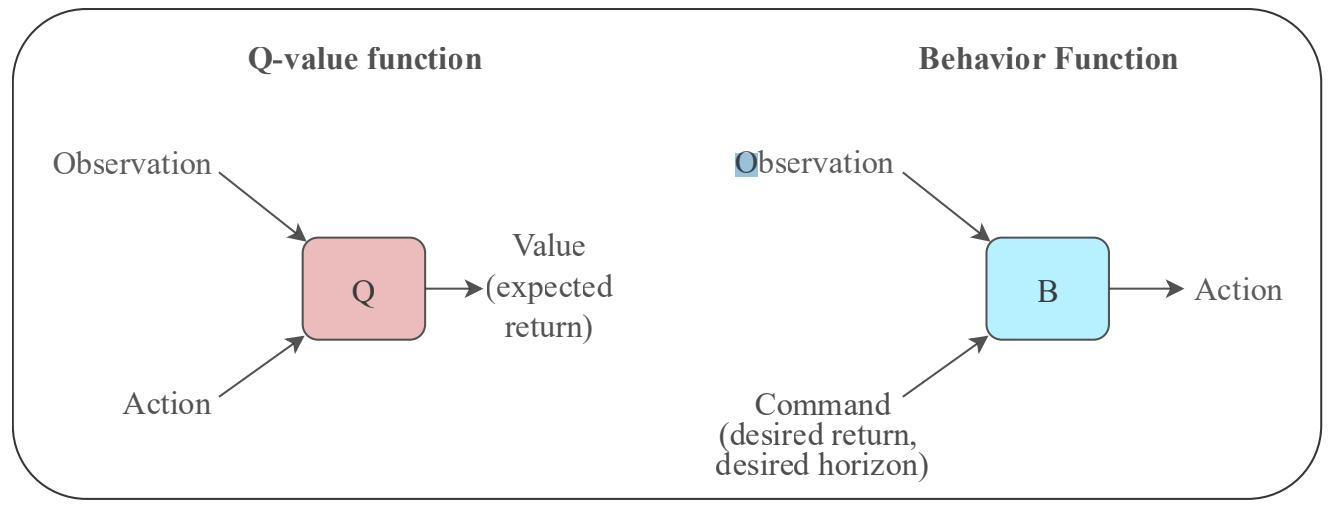
\includegraphics[scale=.42]{img/udrl_graphic.PNG}
\caption{Key distinction between traditional RL and UDRL: the roles of actions and returned are switched while UDRL can have additional command inputs. Image from \citep{srivastava2019training}.}
\end{figure*}


\begin{figure*}[ht]
\centering
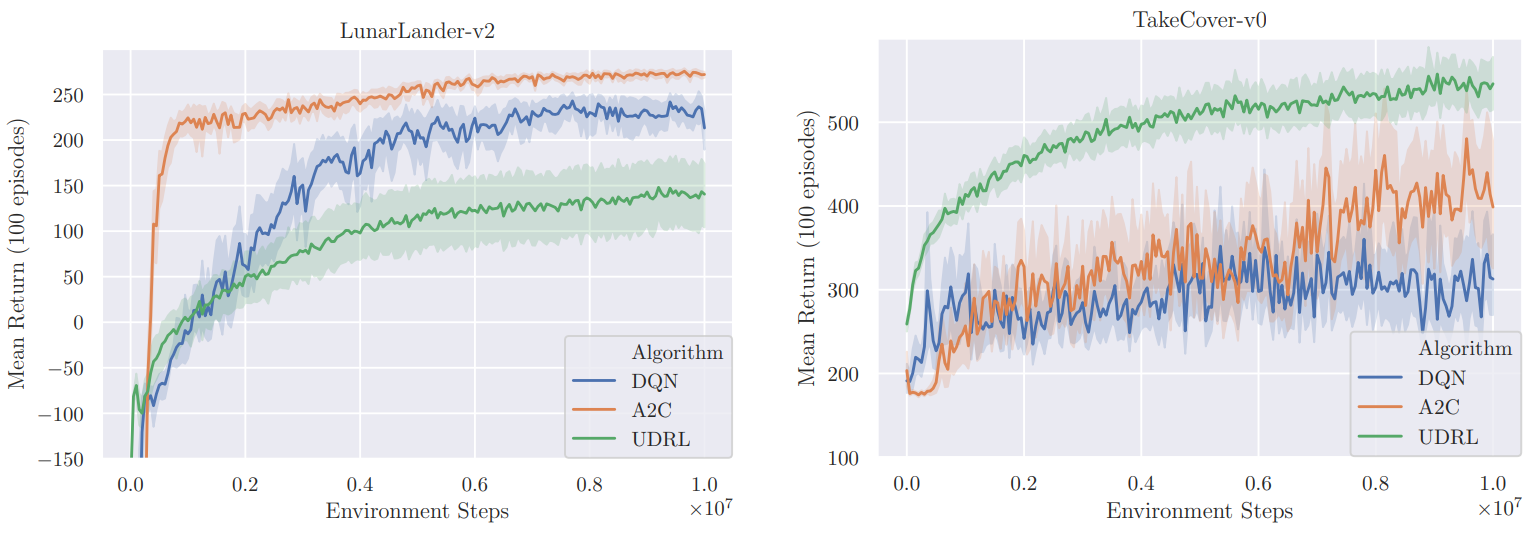
\includegraphics[scale=.39]{img/udrl_test_image.PNG}
\caption{\citet{srivastava2019training} tested a pilot implementation of UDRL against the more traditional Deep Q-Learning (DQL) and an Advantage ACtor-Critic (A2C, from \citep{mnih-2015}) on two test environments well known for RL: LunarLander-v2 and TakeCover-v0, available in the Open AI Gym and VizDoom \citep{openaigym, vizdoom}, graphs from \citep{srivastava2019training}.}
\end{figure*}
\newpage

\cite{schmidhuber2019reinforcement} also introduced an approach for teaching a robot to imitate humans, based on the Imitate-Imitator concept after which parents imitate the babbling of their babies and use child-directed speech: robots learn through supervised learning how humans imitate the robots' current behaviour by mapping a video which functions as input commands. Afterwards, they were supposed to generalise and imitate videos of humans executing new behaviour. This model could be applied to any sequential or multi-modal sensory data (including spoken commands or gestures) from which the desired behaviour can be described to an RNN. The first step is to describe the robot's current behavior 


\section{Problems for NLP in RL}
Research faces a few problems regarding the application of RL in NLP. 

While most research focuses on the reward function in order to maximise the agent's expected long-term reward, \citet{madureira2020} discussed the importance of \textbf{state} in RL for NLP. While the formalisation of the state and its properties depends on the value and reward function, there is less attention directed towards the state. This shows for example in the fact that many researchers neglect describing their state signal and the reasoning of their choice, which alone makes understanding and replicating their models more difficult. With the rise of neural network models in RL for NLP, states could be more easily represented by a vector and thus more easily fed into the value or policy function. \citet{madureira2020} appealed for more linguistically interpretable and grounded state representations next to encouraging researchers to pay more attention to the choice of their state function, its explanation and respective evaluation in the paper. While this seems to be especially problematic for the state, the lack of detailed description can span across all parts of RL research.

\subsection{Data and Language}
\textbf{Anglocentrism} dominates most research fields, with NLP and more specifically RL being no exception. This is due to English continuing to be the main language in which research is written and communicated. While this is not a problem per se, it compels many researchers to also use English as their main language for conducting their experiments due to available data and funding for English research. This homogeneity is a common property of a young research field but still needs to be overcome by broadening up to other languages. This is not only important in terms of ethical diversity but also a necessary step to achieve overall application of RL across languages. \\\\
\textbf{Data} is not only limited in language but also in size and diversity. Since RL models tend to improve by larger corpora, it becomes exponentially difficult to provide datasets of sufficient quality by increase of size. Consequently, many experiments are performed on the same datasets and thus in the same language. The few studies that concern languages other than English commonly exploit machine translation, for example between English and German \citet{yasui-etal-2019}. \\\\
Some newer and more innovative datasets have not been created specifically for training RL models but can be exploited for training them, such as the SCONE (Sequential CONtext-dependent Execution) introduced by \citet{long-2016} and applied to RL by \cite{guu-etal-2017-language}. It spans three different domains which do not include semantic annotations but only world states. Therefore it makes training ambiguous while the RL agent develops a strategy to navigate the "Alchemy", "Tangrams" and "Scene" problems.\\\\
Projects like Amazon Mechanical Turk and DefinedCrowd help with providing larger datasets generated and annotated by humans  for different purposes since it allows researchers to have access to a large and diverse population \citep{AMTurk-2012,DefinedCrowd}. 

\subsection{Knowledge Representation}
It is not only crucial for science in which language data is available but also how language is generally implemented in the other parts of an RL agent. Knowledge representation describes how real-life (or human) knowledge is encoded (=represented) in a way that a machine understands it and can use it to solve complex problems. An example of knowledge representation is the encoding of pictures or language.
\par

\textbf{Grounding} ---connecting or relating language to the real world--- is dependent on the representation of knowledge and will become one of the key features in future RL research according to \citet{narasimhan-2018}. While language needs to be encoded in a way that an RL agent can utilise it, the balance between modifying language and leaving it in its natural state such that the bridge between RL agents and the real world can be crossed. Advancing methods for grounding could make a significant different for real life applications or RL in NLP as well as give new linguistic insights.

\subsection{Evaluation measures}
The choice of evaluation measures is especially problematic in RL agents that generate language. On one hand, automating evaluation is complex and unreliable but on the other hand, human evaluation is very inefficient in time and resources. Some attempts have been made to combine both approaches, although not in the domain of RL but in a neural paraphrasing model \citep{goyal-durrett-2020-neural} by simply applying both a quantitative and a human evaluation on the data and combining the scores. There is another novel attempt to improve the Bilingual Evaluation Understudy (BLEU) and make it more robust for human judgement, called Bilingual Evaluation Understudy with Representations from Transformers (BLEURT) \citep{papineni-etal-2002-bleu,sellam2020bleurt}. BLEURT generalises the model in pre-training with millions of synthetic examples. The authors claim that their model is robust and reaches an unprecedented level of quality which is closer to human evaluation than previous models.\\\\
Motivated by the instability of automatic evaluation methods for NLG (although used in 80\% if empirical papers presented at the ACL track on NLG or INLG in 2018 versus 3\% using extrinsic human evaluation), \citet{van-der-lee-etal-2019-best}, there is no consensus yet of how (NLG) systems should be evaluated by humans. They argue against automated metrics with their uninterpretability and that they do not correlate with human evaluation. In their paper, they give an overview over existing human evaluation models and summarise a set of best practices for human evaluation in NLG.\\\\

\begin{table*}[ht]
\begin{center}
\begin{tabular}{  m{4em}  m{12cm} }
 \textbf{Topic} & \textbf{Best practice}  \\ \hline
 General & Always conduct a human evaluation (if possible).  \\  \hline
 Criteria & Use separate criteria rather than an overall quality assessment.
Properly define the criteria that are used in the evaluation. \\\hline
Sampling & Preferably use a (large-scale) reader-focused design rather than a (small-scale) expert-focused design.
Always recruit sufficiently many participants. Report (and motivate) the sample size and the demographics. \\\hline
Annotation &  For a qualitative analysis, recruit multiple annotators (at least 2, more is better)
Report the Inter-Annotator Agreement score with confidence intervals, plus a percentage agreement. \\\hline
Measurement & For a quantitative study, use multiple item 7-point (preferably) Likert scales, or (continuous) ranking. \\\hline
Design &  Reduce order- and learning effects by counterbalancing/random ordering, and properly report this. \\\hline
Statistics & If the evaluation study is exploratory, only report exploratory data analysis.
If the study is confirmatory, consider preregistering and conduct appropriate statistical analyses.
\end{tabular}
\caption{List of best practices for human evaluation of automatically generated text from \citet{van-der-lee-etal-2019-best}.}
\label{table:1}
\end{center}
\end{table*}
Although introduced in 2002 or shortly after, many recent studies still evaluate with the \textbf{BLEU}, \textbf{Recall-Oriented Understudy for Gisting Evaluation (ROUGE)} or \textbf{Metric for Evaluation of Translation with Explicit ORdering (METEOR)} \citep{lin-2004-rouge, banerjee-lavie-2005-meteor} despite new ways of evaluating being introduced, for example by the yearly metrics challenge by the WMT conference \citep{SIGMT-2020}. While there is evidence for BLEU's validity in predicting human judgements \citep{reiter-2018-astructured}. However, it has been stated BLEU and similar evaluation methods are outdated and should not be used for evaluating Natural Language Generation \citep{reiter-2020-small, reiter-2020-why, reiter-2018-astructured, mathur-etal-2020-tangled}. This is because BLEU is checking for matching ngrams in generated and texts written or annotated by humans. With the evolution of Machine Translating, variation of text becomes more important, which is not what BLEU is optimised for. A well varied text would decrease ratings from BLEU and similar metrics which reward systems which consistently use a specific wording and syntax. Hence, human preference is the opposite of BLEU's preference. BLEU also tends to perform worse on models that use languages like German in Machine Translation or other NLP applications for a similar reason: the word order in German is relatively free compared to English and Romance languages which impacts the reliability of BLEU \citet{reiter-2018-bleu}.\\\\
Next to the older BLEU or STS score, new approaches have been tested to \textbf{automatise evaluation}: \citet{yasui-etal-2019} trained a BERT-model to recognise semantically similar sentences of a translation model. Here we see that machine translated sentences can achieve human performances, but human translation is still superior when it spans more than one sentence. \\\\ 
In paraphrase generation, \citet{li-etal-2018-paraphrase} proposed \textbf{training their own evaluators} (together with a generator) by two different models, Reinforced by Matching-Supervised Learning (RbM-SL) and Reinforced by Matching-Inverse Reinforcement Learning (RbM-ISL). The method reminds of General Adversarial Networks (GANs) with the difference being that "GANs employ the discriminator to distinguish generated examples from real ones while RbM-IRL employs the evaluator as a reward function in RL. The generator in GAN is trained to maximise the loss of the discriminator in an adversarial way, while the generator in RbM-IRL is trained to maximize the expected cumulative reward from the evaluator". Each models perform better at a different task: RbM-SL performs better on a Quora dataset because it can make use of the additional labelled data to train the evaluator. RbM-IRL performs better on the Twitter data because its evaluator deals better with a smaller data than its counterpart, thus RbM-SL scores better on the relevancy measure and RbM-IRL better on fluency.

\section{Conclusion}
As  \citet{ijcai2019} stated, "approaches combining language and RL will find applications as wide-ranging as autonomous vehicles, virtual assistants and household robots". While RL in NLP has made some advances, it is still far from being successfully exploited in Life Sciences. More careful research, especially in regard to the limitations and ethical implications, has to be conducted in order to model agents who can reliably applied to everyday life. \\\\
More datasets of high quality and large size which are free of charge might improve future studies and make research more accessible. Projects like Amazon Mechanical Turk and DefinedCrowd opened a new door for research but are still hidden behind a paywall which is a disadvantage for research because not everybody who would want to work with the data is able to.

\newpage
\bibliography{bib}

\end{document}